\documentclass[11pt, a4paper]{article}

\usepackage{listings}
\usepackage{color}
\usepackage[normalem]{ulem}
\usepackage{graphicx}
\usepackage{hyperref}


\definecolor{dkgreen}{rgb}{0,0.6,0}
\definecolor{gray}{rgb}{0.5,0.5,0.5}
\definecolor{mauve}{rgb}{0.58,0,0.82}

\lstset{frame=tb,
  language=SQL,
  aboveskip=3mm,
  belowskip=3mm,
  showstringspaces=false,
  columns=flexible,
  basicstyle={\small\ttfamily},
  numbers=none,
  numberstyle=\tiny\color{gray},
  keywordstyle=\color{blue},
  commentstyle=\color{dkgreen},
  stringstyle=\color{mauve},
  breaklines=true,
  breakatwhitespace=true
  tabsize=3
}

\begin{document}
\title{}
\author{Groep A\\ Eindrapport}
\date{27 mei 2014}
\maketitle

\section{Status}
Het project is afgewerkt. Alle verplichte functionaliteit is aanwezig en we hebben heel wat extra functionaliteit voorzien. De database is goed gevuld met meer dan 90.000 entries. De afgewerkte versie van de website staat online op \url{www.coachcenter.be} / \url{www.coachcenter.net} en blijft automatisch up to date met de recentste data.
\section{Taakverdeling}
In deze sectie noemen we enkel de grote onderdelen waar we veel aan werkten. Dit is verre van een complete lijst. Voor een vollediger beeld is er het overzicht van de commits op onze git repository \\ \url{https://github.com/rubenvanassche/Programming-Project-Databases}
\subsection{Stijn}
Was verantwoordelijk voor het binnenhalen alle voetbalgerelateerde data (door middel van crawler); dit omvatte matchen (zowel de nog te spelen als de gespeelde), competities, info over de matchen zoals spelers, kaarten, doelpunten, en spelerwissels, teams en zijn spelers, FIFA rank,... Uiteraard zou de design voldoende robuust moeten zijn en bovendien effici\"ent genoeg zodat het geen eeuwigheid zou duren om de net gespeelde matchen up-to-date te brengen.
\subsection{Kristof}
Heeft enkele pagina's gemaakt en ook de back-end verzorgd die nodig was voor die pagina's. Heeft de basis gelegd voor user profiles en heeft private usergroups gemaakt. Bouwde een notificatiesysteem en zorgde ook voor de email reminders.
\subsection{Tom}
Maakte de algoritmen die aan de hand van de data in de database een beredeneerde calculatie moest maken over de uitslag van de wedstrijden.
Zorgde voor het sorteersysteem en filtersysteem van de tabellen.
\subsection{Jakob}
Maakte een gebruikerssysteem (registreren en inloggen). Maakte een interactieve wereldkaart met FIFA scores. Bouwde het betsysteem uit. Maakte een visualisatie van statistieken uit de database.
\subsection{Ruben}


\section{Design}
TODO: LAMP, Laravel, Bootstrap
\subsection{Voorspellingsalgoritme}
Het voorspellingssysteem hebben wij opgesplitst in 2 essenti\"ele delen, namelijk het voorspellen van een winnaar van een wedstrijd, en het bepalen van de te verwachten score. Factoren die wij belangrijk vonden om rekening mee te houden in het voorspellen van dit alles zijn vooral resultaten van onderling eerder gespeelde wedstrijden, en gemiddeldes van andere wedstrijden tegen andere ploegen. Ook wordt altijd rekening gehouden met de locatie waar gespeeld wordt (uit of thuis).
\\
\\
Het voorspellen van de winnaar is natuurlijk de makkelijkste van de twee. We beginnen simpelweg door te kijken naar eerder gespeelde wedstrijden tussen deze ploegen. We werken met een puntensysteem waarbij een ploeg punten krijgt wanneer het een wedstrijd wint. Hierbinnen maken we ook nog eens het onderscheid of de set-up uit/thuis dezelfde is of omgekeerd. Voor elke match met dezelfde set-up krijgt de winnende ploeg 1 punt, met een omgekeerde set-up 0.9.
Daarna gaan we kijken naar algemene resultaten, maar weer rekening houdende met het al dan niet uit/thuis spelen. We kijken naar alle wedstrijden die de thuisploeg thuis speelde, en de uitploeg uit speelde. Hun win/loss ratio wordt bij hun puntentotaal geteld. Vervolgens kijken we naar de wedstrijden waar de thuisploeg uit speelde, en de uitploeg thuis. Hierbij wordt de win/loss ratio vermenigvuldigd met factor 0.9 bij het puntentotaal geteld. Ook gaan we de FIFAscore van elk team gedeeld door 1000 bij het puntentotaal tellen. Tot slot gaan we de punten vergelijken en op basis daarvan kunnen we de kans bepalen dat een bepaalde ploeg wint.
\\
\\
Het bepalen van een score is iets complexer. Dit volgt een gelijkaardig systeem als hierboven, maar met een belangrijk verschil. Hier werken we niet met het optellen van punten, maar wel met gemiddeldes. We kijken terug naar de vier zelfde situaties, maar gaan nu het gemiddelde aantal doelpunten per match berekenen. Hiervan nemen we het gewogen gemiddelde (gewichten 1, 0.9, 0.7 en 0.5). Dit is dan de voorspelde uitkomst van de match. Indien deze uitkomst niet overeenkomt met de voorspelde winkansen, wordt de score aangepast. Merk op dat het werken met gemiddeldes betekent dat de voorspelde uitkomsten vaak redelijk weinig goals omvatten.
\\
\\
Eerst waren we ook van plan om nog meer dingen te laten berekenen aan de hand van de data die we hebben. Al snel bleek dat deze dingen vaak te willekeurig zijn en daarom konden er ook niet echt beredeneerde gokken over worden gemaakt. Er zijn inderdaad wel spelers die vaker kaarten krijgen dan anderen, maar uiteindelijk blijkt dit toch veelal willekeurig te zijn. Al snel bleek dat een algoritme hiervoor vaker ernaast zou zitten dan erop. Om onze gebruiker dan ook niet het valse gevoel te geven van hierop te kunnen gokken aan de hand van dit algoritme, hebben we besloten het niet in het uiteindelijke project te steken.


\section{Database}
Onze database bestaat 12 tabellen met voetbalgerelateerde data en 8 usergerelateerde tabellen.
\begin{enumerate}
\item 'continent': Tabel voor werelddelen. Bevat een id en een naam.
\item `country`: Tabel voor landen. Bevat een id, een naam, de id van het werelddeel waarin het land ligt, en een afkorting voor de naam van het land. Die afkorting zal gebruikt worden op de website.
\item `player`: Tabel voor voetbalspelers. Bevat een id, een naam en een boolean die aangeeft of de speler geblesseerd is.
\item `coach`: Tabel voor voetbalcoaches. Bevat een id en een naam.
\item `team`: Tabel voor voetbalteams. Bevat een id, een naam, een id van het land van het team, een id van de huidige coach van het team en de FIFA score.
\item `competition`: Tabel voor voetbalcompetities. Bevat een id en een naam.
\item `match`: Tabel voor voetbalmatches. Bevat id's van thuis- en uitteam, id van de competitie en een datum.
\item `playerPerTeam`: Tabel die spelers en teams met elkaar linkt. Bevat id's van een speler en een team.
\item `playerPerMatch`: Tabel die spelers en matches met elkaar linkt. Bevat id's van een speler en een match en de tijden waarop de speler op het veld kwam en van het veld ging.
\item `teamPerCompetition`: Tabel die teams en competities met elkaar linkt. bevat id's van een team en een competitie.
\item `goal`: Tabel voor doelpunten. Bevat id van match waarin doelpunt gescoord is, tijdstip waarop, id van de speler die het doelpunt scoorde, id van het team waarnaar het punt ging en een boolean die aangeeft of het doelpunt tijdens de penaltyfase gescoord werd.
\item `cards`: Tabel voor gele en rode kaarten. Bevat een id, een id van de speler die de kaart kreeg, een id van de match waarin de kaart gegeven werd, de kleur van de kaart en de tijd waarop de kaart gegeven werd.
\item `user`: Meer uitleg bij sectie over gebruikers.
\item `bet`: Meer uitleg bij sectie over voorspellingen
\item `notifications`: Meer uitleg bij sectie over notifications
\item `userGroup`: Meer uitleg bij sectie over user groups
\item `userGroupInvites`: Meer uitleg bij sectie over user groups
\item `userGroupMessages`: Meer uitleg bij sectie over user groups
\item `userGroupMessagesContent`: Meer uitleg bij sectie over user groups
\item `userPerUserGroup`: Meer uitleg bij sectie over user groups

\end{enumerate}

\subsection{ER-diagramma}
Zie laatste pagina
\subsection{Relational model}
continent(\uline{id}, name) \\
country(\uline{id}, name, continent\_id, abbreviation) \\
player(\uline{id}, name) \\
coach(\uline{id}, name) \\
team(\uline{id}, name, country\_id, coach\_id, fifapoints, twitterAccount) \\
competition(\uline{id}, name) \\
match(\uline{id}, hometeam\_id, awayteam\_id, competition\_id, date) \\
playerPerTeam(\uline{player\_id}, \uline{team\_id}, position) \\
playerPerMatch(\uline{player\_id}, \uline{match\_id}, intime, outtime) \\
teamPerCompetition(\uline{team\_id}, \uline{competition\_id}) \\
goal(match\_id, time, player\_id, team\_id) \\
cards(\uline{id}, player\_id, color, time) \\
user(\uline{id}, facebookid, username, firstname, lastname, email, password, country\_id, session\_id, registrationcode, betscore, about, receive\_email, age, picture) \\
bet(\uline{id}, user\_id, match\_id, hometeam\_score, awayteam\_score, first\_goal, hometeam\_yellows, hometeam\_reds, awayteam\_yellows, awayteam\_reds, evaluated, betdate) \\
notifications(\uline{id}, actor\_id, subject\_id, object\_id, type\_id, status, created\_date, updated\_date) \\
userGroup(\uline{id}, name, private, created) \\
userGroupInvites(\uline{id}, user\_id, usergroup\_id, invitedby\_id, created) \\
userGroupMessages(\uline{id}, usergroup\_id, user\_id, title, created) \\
userGroupMessagesContent(\uline{id}, user\_id, message\_id, content, created) \\
userPerUserGroup(\uline{user\_id}, \uline{usergroup\_id}, created)\\

\subsection{Constraints}
\begin{lstlisting}
-- Constraints for table `cards`
--
ALTER TABLE `cards`
  ADD CONSTRAINT `match` FOREIGN KEY (`match_id`) REFERENCES `match` (`id`) ON DELETE NO ACTION ON UPDATE CASCADE,
  ADD CONSTRAINT `player` FOREIGN KEY (`player_id`) REFERENCES `player` (`id`) ON DELETE CASCADE ON UPDATE CASCADE;

--
-- Constraints for table `country`
--
ALTER TABLE `country`
  ADD CONSTRAINT `continent` FOREIGN KEY (`continent_id`) REFERENCES `continent` (`id`);

--
-- Constraints for table `goal`
--
ALTER TABLE `goal`
  ADD CONSTRAINT `goal_match` FOREIGN KEY (`match_id`) REFERENCES `match` (`id`) ON DELETE NO ACTION ON UPDATE CASCADE,
  ADD CONSTRAINT `goal_player` FOREIGN KEY (`player_id`) REFERENCES `player` (`id`) ON DELETE NO ACTION ON UPDATE CASCADE,
  ADD CONSTRAINT `goal_team` FOREIGN KEY (`team_id`) REFERENCES `team` (`id`) ON DELETE NO ACTION ON UPDATE CASCADE;

--
-- Constraints for table `match`
--
ALTER TABLE `match`
  ADD CONSTRAINT `awayteam` FOREIGN KEY (`awayteam_id`) REFERENCES `team` (`id`) ON DELETE CASCADE ON UPDATE CASCADE,
  ADD CONSTRAINT `hometeam` FOREIGN KEY (`hometeam_id`) REFERENCES `team` (`id`) ON DELETE CASCADE ON UPDATE CASCADE,
  ADD CONSTRAINT `match_competition` FOREIGN KEY (`competition_id`) REFERENCES `competition` (`id`);

--
-- Constraints for table `playerPerMatch`
--
ALTER TABLE `playerPerMatch`
  ADD CONSTRAINT `player_per_match` FOREIGN KEY (`match_id`) REFERENCES `match` (`id`) ON DELETE CASCADE ON UPDATE CASCADE;

--
-- Constraints for table `playerPerTeam`
--
ALTER TABLE `playerPerTeam`
  ADD CONSTRAINT `player_per_team` FOREIGN KEY (`team_id`) REFERENCES `team` (`id`) ON DELETE CASCADE ON UPDATE CASCADE;

--
-- Constraints for table `team`
--
ALTER TABLE `team`
  ADD CONSTRAINT `team_coach` FOREIGN KEY (`coach_id`) REFERENCES `coach` (`id`) ON DELETE NO ACTION ON UPDATE CASCADE,
  ADD CONSTRAINT `team_country` FOREIGN KEY (`country_id`) REFERENCES `country` (`id`);

--
-- Constraints for table `teamPerCompetition`
--
ALTER TABLE `teamPerCompetition`
  ADD CONSTRAINT `tpc_competition` FOREIGN KEY (`competition_id`) REFERENCES `competition` (`id`);

  --
-- Constraints for table `bet`
--
ALTER TABLE `bet`
  ADD CONSTRAINT `matchID` FOREIGN KEY (`match_id`) REFERENCES `match` (`id`) ON DELETE CASCADE ON UPDATE CASCADE,
  ADD CONSTRAINT `userID` FOREIGN KEY (`user_id`) REFERENCES `user` (`id`) ON DELETE NO ACTION ON UPDATE CASCADE;

\end{lstlisting}

\section{User interface}

Hoewel Laravel beschikt over een volledig uitgewerkt loginsysteem, besloten we ons eigen systeem te schrijven. Een dergelijk systeem gebruikt een database voor het opslaan van users, dus is het niet meer dan logisch dat we dit in een vak met betrekking tot databases zelf gaan programmeren. In de database bestaat een tabel 'user', met als fields 'id', 'username', 'firstname', 'lastname', 'email', 'password', 'country\_id', 'session\_id', 'registrationcode', 'betscore', 'about', 'receive\_email', 'age' en 'picture' . De id is een auto incrementing integer die dient als key voor elke entry van de tabel. We voorzien een username, zodat gebruikers niet noodzakelijk hun echte naam moeten prijsgeven. Daarnaast is het een makkelijke manier om gebruikers op de website een unieke benaming te geven. Voornaam en familienaam zijn apart opgeslagen, zodat we in bijvoorbeeld emails gebruikers niet altijd met hun volledige naam niet hoeven aan te spreken. Het paswoord is uiteraard gehasht opgeslagen. Het hashen gebeurt via Laravel, aan de hand van bcrypt. Bcrypt is gebaseerd op het Blowfishalgoritme en heeft een salt ingebouwd, wat accounts beschermt tegen aanvallen gebruik makende van rainbow tables. Laravel biedt een functie voor het vergelijken van een ongehasht en gehasht paswoord. Verder vragen we gebruikers ook in welk land ze wonen en wat hun leeftijd is. De session\_id wordt gebruikt om bij te houden of een gebruiker ingelogd is. We plaatsen een tijdelijke cookie met hetzelfde id bij de gebruiker, en kunnen dit zo nagaan. De registratiecode wordt gebruikt bij het nagaan van de validiteit van het emailadres van een gebruiker. De registratiecode wordt gemaild naar de gebruiker, en het account wordt pas geactiveerd wanneer deze code ingegeven wordt. De betscore houdt bij hoe goed een gebruiker presteert bij het gokken. De gebruiker kan een korte beschrijving van zichzelf geven, die in 'about' wordt opgeslagen. 'Receive\_email' is een boolean die bijhoudt of de gebruikers herinneringse-mails voor wedstrijden waar hij nog niet op gokte wil krijgen. Ten slotte bevat 'picture' de profielafbeelding van de gebruiker.
\\
\\
Voor de validatie van input bij registreren (zijn verplichte velden ingevuld, staat bij emailadres wel een emailadres, is tweemaal hetzelfde paswoord ingetypt, ...) is de validatie van Laravel gebruikt. Dergelijke validatiecode ziet er heel wat beter uit voor de programmeur dan via een hoop simpele if-statements en reguliere expressies. We gebruiken de Laravel Query Builder voor makkelijker schrijven van SQL queries niet, dit gebeurt zoals opgegeven met ruwe SQL queries.
\\
\\
Op elke webpagina verschijnt voor een niet-ingelogde gebruiker een loginknop. Het loginmenu wordt dan over de huidige pagina (in een 'modal', een feature van Bootstrap) weergegeven. Indien de gebruiker met foute gegegvens probeert in te loggen, wordt dit afgehandeld in diezelfde modal. Eens inloggen succesvol is, verschijnt er in de modal nog een bericht om het inloggen te bevestigen. Eens dat weggeklikt wordt, bevindt de gebruiker zich terug op dezelfde pagina als voorheen. Er is ook een knop "forgot password", die de gebruiker naar een nieuwe pagina leidt. De gebruiker geeft zijn emailadres in, en er wordt een email gestuurd waarmee het paswoord gereset kan worden. Indien men probeert in te loggen met een account waarvan het emailadres nog niet gevalideerd is, verschijnt een knop om de activatiemail opnieuw te versturen. \\ Bij een ingelogde gebruiker wordt bij elke bezochte pagina de login cookie gerefresht, zodat een gebruiker bij langdurige sessies op de site niet om de zoveel tijd opnieuw hoeft in te loggen. \\ \\

TODO: Facebooklogin \\ \\

Eens ingelogd, worden de registratie- en inlogknoppen vervangen door "My Profile", "Bets", "Preferences" en "Logout". \\
"My Profile" is een pagina waarop wat persoonlijke informatie als land en bet score te zien zijn. Deze pagina is voor iedereen, zelfs niet-ingelogde gebruikers zichtbaar. Enkel op je eigen profiel verschijnen nog de tabs "Notifications", "My Groups" en "Invitations". Op deze functionaliteit wordt verder ingegaan in andere secties. \\
Onder "Preferences" is het mogelijk je persoonlijke gegevens aan te passen.	Ook is er een opt-out voor herinneringsemails omtrent bets. Uploaden van profielafbeeldingen gebeurt ook daar.
Als de gebruiker op "logout" klikt, wordt hij uitgelogd en naar de homepage gestuurd. \\ \\

Uitgelogde gebruikers zullen niet gelinkt worden naar pagina's voor enkel gebruikers. Indien iemand toch probeert een dergelijke pagina te bezoeken door de URL in te typen, zal hij gevraagd worden eerst in te loggen of te registreren en de eigenlijke pagina niet te zien krijgen. \\ \\

\subsection{Betsysteem}
Gebruikers kunnen pronostieken invullen voor matchen in de toekomst. Voor een ingelogde gebruiker verschijnt op matchpagina's een knop genaamd "bet", zolang de gebruiker nog niet eerder een gok heeft uitgebracht op die match. Wanneer de gebruiker erop klikt, verschijnt het betformulier in een modal. De gebruiker is verplicht om een eindscore in te vullen. Verder kan de gebruiker ook nog voorspellen welk team de eerste goal scoort en hoeveel kaarten van elke soort elk team zal krijgen. Deze opties zijn echter allemaal optioneel. De gok wordt geregistreerd van zodra er op "bet" geklikt wordt. Elke gebruiker heeft per match slechts \'e\'en kans per match, denk dus goed na over je bet. Een overzicht van gemaakte bets kan gevonden worden via "bets" in de bovenste balk op de website. Daar worden bets opgedeeld in bets op toekomstige matchen en bets op verleden matchen. Er kan telkens doorgeklikt worden naar de matchen en teams. \\ \\
Eens een match gespeeld is, worden de bets erop binnen de drie uur ge\"evalueerd. Aan elke gebruiker wordt een aantal punten toegekend. Dat puntentotaal kan ook negatief zijn. Er kan met elke gemaakte gok een aantal punten gewonnen of verloren worden. Er kunnen altijd meer punten gewonnen worden dan verloren. Eerst hadden we het idee om correcte riskante gokken meer punten waard te maken. We waren van plan om "riskante gokken" te defini\"eren als keuzes waar weinig gebruikers voor gingen. Realistisch gezien zullen er waarschijnlijk niet erg veel gebruikers actief zijn tijdens het WK 2014 en zou een dergelijk systeem niet erg veel nut hebben. Daarom hebben we per optie een vast aantal punten toegekend (maar niet voor elke optie evenveel). \\ \\

\subsection{Filter- \& sorteersysteem}
Ook kunnen gebruikers zowat elke tabel die te vinden is op de website sorteren zoals zij dit zelf willen. Dit hebben we verwezenlijkt met een slim stukje javascript dat een uitbreiding is op tablesorter. Hierdoor moet de webpagina niet opnieuw geladen worden. Ook is er een ingebouwd filter systeem waardoor de gebruiker op een overzichtelijke en snelle manier ervoor kan zorgen dat alleen de data die hij relevant is voor hem zichtbaar is. Dit is ge\"implementeerd aan de hand van een zoekbalk. We hebben die zoekbalk enkel geplaatst op de pagina met alle teams. Andere tabellen zijn niet groot genoeg om een filter voor nodig te hebben. We hebben besloten om geen lijst van alle matchen in heel de database op de website te zetten; dit zou te onoverzichtelijk worden. In de plek kan de gebruiker uit een lijst van alle competities een competitie (telkens van slechts 1 jaar) kiezen en daarvan alle matchen zien. Daarin is ook te zien in welke fase van de competitie elke match gebeurde, indien deze data beschikbaar is.
Al deze functionaliteit zou moeten bijdragen aan de gebruiksvriendelijkheid van de website. Ook hebben we dit alles zo intu\"itief mogelijk gehouden zodat de gebruiker zonder enig probleem kan navigeren over de website en zich meer kan concentreren op de inhoud dan hoe hij daar moet geraken.



\subsection{Notificaties}
Ook is er in ons systeem een uitgebreid notificatiesysteem aanwezig. Wanneer een gebruiker ingelogd is, zal er bovenaan naast het user menu een nieuw item tevoorschijn komen (icoon: ster). Op het moment dat er een notificatie is voor de gebruiker wordt die hier getoond. Zonder op het item te klikken kan je al zien hoeveel ongelezen notificaties je hebt door het cijfer in superscript dat naast het sterretje staat. Als de gebruiker hierop klikt komt er een dropdown menu tevoorschijn met de meest recente notificaties. Deze notificaties linken naar de relevante pagina. \\
Om dit mogelijk te maken is er een notificatiesysteem geschreven dat gemakkelijk uitbreidbaar is. Elke notificatie heeft een specifiek formaat: er is altijd een actor, een subject, een object en een type. Aan de hand van deze informatie kan er dan een gepaste boodschap worden getoond.
\begin{enumerate}
\item Actor: de uitvoerende partij
\item Subject: de persoon voor wie de notificatie bestemd is
\item Object: de specifieke informatie over de notificatie
\item Type: om duidelijk te maken welk voor type notificatie we hebben (Bijvoorbeeld een usergroup invite)
\end{enumerate}
\subsubsection{Implementatie}
Elke notificatie komt dus overeen met een rij van de notifications table. Wanneer een notificatie wordt opgeslagen (Notifications::saveNotification) komt er niet veel bij zien: gewoon letterlijk de kolommen invullen.
Bij het opvragen van een notificatie (Notifications::getNotification) komt er wat meer bij kijken: in het resultaat wordt de informatie van het object erbij gezet.
Wanneer er op de notificatie wordt geklikt wordt de redirect methode van de NotificationController opgeroepen die naargelang het type notificatie de gebruiker naar de juiste pagina redirect.

\subsection{Soorten notificaties}
\subsubsection{Usergroup invites}
Een gebruiker nodigt een andere gebruiker uit om een usergroup te joinen.
\begin{enumerate}
\item Actor: de gebruiker die de persoon uitnodigt
\item Subject: de uitgenodigde gebruiker
\item Object: de userGroupInvite
\item Type: 1, Notifications::INVITE\_USER\_GROUP
\end{enumerate}
De notificatie zal linken naar de gebruiker zijn profiel waar die de invitatie zal kunnen accepteren of weigeren.

\subsubsection{Remind user bets}
Het systeem herinnert de gebruikers om te betten op matchen waar ze dat nog niet op hebben gedaan.
Omdat het systeem dit verstuurt zullen we de actor en subject dezelfde personen nemen.
\begin{enumerate}
\item Actor: de gebruiker
\item Subject: de gebruiker
\item Object: NULL (Geen verdere info nodig)
\item Type: 2, Notifications::REMIND\_USER\_BETS
\end{enumerate}
De notificatie zal linken naar de upcoming matches page, waar de gebruiker gemakkelijk kan zien op welke matches hij/zij nog niet op heeft gebet.

\subsubsection{Nieuwe discussie in usergroup}
Wanneer een gebruiker een nieuwe discussie start in een usergroup zullen alle members van die groep een notificatie hierover krijgen.
\begin{enumerate}
\item Actor: de gebruiker die de discussie heeft aangemaakt
\item Subject: een gebruiker die lid is van de groep
\item Object: de discussie
\item Type: 3, Notifications::NEW\_DISCUSSION
\end{enumerate}
De notificatie zal linken naar de discussie.

\subsubsection{Nieuwe reply in discussie}
Als een gebruiker een bericht post in de discussie zullen alle deelnemers van die discussie hierover genotified worden.
\begin{enumerate}
\item Actor: de gebruiker die een nieuwe reply heeft gemaakt
\item Subject: deelnemer aan de discussie
\item Object: discussie
\item Type: 4, Notifications::NEW\_MESSASGE
\end{enumerate}
De notificatie linkt naar de discussie.

\subsection{Email reminders}
Gebruikers worden tijdig herinnerd wanneer ze nog niet op bepaalde wedstrijden hebben gebet. Dit wordt mogelijk gemaakt door een combinatie van een Laravel command die via een cronjob om de zoveel tijd loopt.
Momenteel worden de gebruikers elke dag herinnerd om te wedden op de wedstrijden die de komende twee dagen worden gespeeld waar ze nog niet reeds hebben op gebet.
Ook wordt er een wekelijks overzicht gegeven op zondag met een overzicht van de wedstrijden die in de komende week worden gespeeld.

De functie die in het Laravel command wordt opgeroepen is de Notifications::sendReminders. Dit zal samen met een email ook een notificatie sturen naar de gebruiker.

Uiteraard moet de gebruiker de mogelijkheid krijgen om geen emails meer te ontvangen. Vandaar dat er ook een opt-out mogelijkheid is. Enerzijds kan je dit doen door op de link in de email te klikken,
anderzijds kan je dit regelen door de knop op de preferences page te gebruiken. Deze knop/link togglet als het ware tussen het ontvangen van email en het niet ontvangen van de mail. Als de gebruiker zich op een later moment
bedenkt kan deze dit dus gewoon via de preferences page (of een link in een email) regelen.

\subsection{User profiles}
Elke geregistreerde gebruiker op CoachCenter heeft zijn eigen profiel. Wanneer een gebruiker zijn eigen profiel bezoekt kan hij zijn notificaties, uitnodigingen en groepen zien.
Ook zijn avatar, betscore, land en `about me` zijn te zien. Hij kan ervoor kiezen zijn profiel te bewerken waarop hij wordt doorgestuurd naar de preferences page.
Op deze preferences page kan een gebruiker zijn passwoord veranderen, van avatar veranderen, emails in- of uitschakelen en andere informatie zoals zijn emailadres, leeftijd en dergelijke aanpassen.
\\
\\
Geregistreerde (en ongeregistreerde) gebruikers kunnen ook de profielen van andere mensen bekijken. Uiteraard zijn nu de notificaties en dergelijke van deze bepaalde gebruiker niet zichtbaar.
Enkel de informatie (avatar, betscore, `about me`, groepen) is zichtbaar.

\subsection{Usergroups}
In de lijst van vereiste functionaliteit stond ook dat er voor ingelogde gebruikers de mogelijkheid moeset zijn om groepen van gebruikers te maken die tegen elkaar kunnen spelen.
Ze moeten scores en ranking binnen een groep kunnen zien en ook moet de mogelijkheid bestaan om andere gebruikers uit te nodigen tot een usergroup.
\\
\\
We hebben twee soorten usergroups gemaakt. Beiden ondersteunen dezelfde functionaliteit maar ze verschillen van elkaar in het opzicht dat de ene soort usergroup publiek is en de andere privaat.
Concreet komt dit erop neer dat in een publieke groep iedereen kan joinen wie wilt (eveneens kan men gebruikers uitnodigen) en in een private groep kunnen enkel mensen joinen die worden uitgenodigd.
\\
\\
De usergroup pagina bevat een tijdslijn waarin events (uiteraard chronologisch geordend) van de groep worden getoond. Zo kan iedereen zien wanneer gebruiker X op welke match heeft gewed, zien wanneer een bepaalde gebruiker is uitgenodigd geweest en is gejoind, ...
Ook worden er discussies ondersteund: dit zijn gesprekken binnen in de usergroup waar iedereen die lid is op kan antwoorden. Wanneer er een nieuwe discussie wordt gestart of wanneer er iemand antwoord in een gesprek waaraan je deelneemt zal je uiteraard een notificatie hierover krijgen.
\\
\\
Bovenaan de usergroup zien we ook de leden met hun betscore ernaast. Zo ontstaat er een soort van competitiedrang die het aantal bets in het systeem alleen maar zal opdrijven.

\subsection{Grafische weergave van statistieken}
Voor de grafische weergave van data gebruiken we Google Charts. Dat biedt heel wat verschillende grafieken. Momenteel zijn op elke teampagina twee grafieken beschikbaar. Er is een taartdiagram dat het percentage gewonnen, verloren en gelijkgespeelde matchen van een team toont. Ook is er een staafdiagram dat het gemiddelde aantal goals en/of kaarten per match per jaar toont. De gebruiker kan kiezen welke combinatie van 'gemiddeld aantal goals', 'gemiddeld aantal gele kaarten' en 'gemiddeld aantal rode kaarten' hij wil zien. De grafiek wordt meteen aangepast, zonder dat de pagina opnieuw geladen moet worden. Deze grafieken bevinden zich onder de tab 'Graphs' op elke teampagina. \\ \\
Op de homepagina staat een grote wereldkaart. De kleur van elk land geeft zijn FIFA score weer. Hoe donkerder het land, hoe hoger de score. Wanneer op een land geklikt wordt, wordt meteen naar de teampagina van het nationale team gelinkt. Voor enkele kleine landen is geen teampagina aanwezig, er gebeurt dan ook niets wanneer erop geklikt wordt. Als op het Verenigd Koninkrijk geklikt wordt, zoomt de kaart in, zodat op de vier aparte delen (Wales, Engeland, Noord-Ierland en Schotland) kan worden geklikt. Deze hebben namelijk elk een apart nationaal team. \\ \\
Ook de voorspellingen van het systeem worden gevisualiseerd. Concreet staat op elke matchpagina van toekomstige matchen een balk in twee kleuren. Het linkerdeel geeft de kans op winst voor de thuisploeg aan, het rechterdeel die voor de uitploeg. Deze balk is niet met Google Charts gemaakt, maar is een progress bar van Bootstrap.
\section{Webpagina's}
De gemaakte webpagina's zijn in het Laravel PHP Framework gemaakt. Dit is een framework dat MVC hoog in het vaandel draagt en dat proberen we dus ook te respecteren.
Elke pagina (View) heeft een controller tot zijn beschikking. Deze dient als tussenstuk tussen het model van de pagina waar de werkelijke queries gebeuren. Over het algemeen is dit wat er gebeurt:
\\
\\
Er wordt een pagina opgevraagd in de url. (Bv. /public/team/1). In de route-file wordt gedefinieerd welke controller er opgeroepen moet worden. Deze controller zal informatie opvragen van het
relevante model en zal deze info doorspelen naar de view van de pagina.
\\
\\
Aanvankelijk was het werken met het framework niet eenvoudig maar eens het wat duidelijker werd zagen we de waarde ervan in.
Het design hebben we grotendeels te danken aan Twitter Bootstrap. Een website ziet er zo relatief gemakkelijk goed uit.
\\
\\
\subsection{Home page}
Bestaat uit 3 tabellen, een news foto feed en een wereldkaart die de landen kleurt in functie van hun WK-ranking.
De 3 tabellen bevatten data over de laatst gespeelde matchen, de opkomende matchen en de fifa-ranking.
\\
De foto newsfeed is een RSS feed van FIFA die we met SimplePie hebben geparsed.
\\
Op de wereldkaart wordt verder ingegaan bij "Grafische weergave van statistieken".
\subsection{Search bar / search results}
Rechtsbovenaan alle pagina's staat een searchbar waarin je een zoekterm kunt invullen en die de beschikbare info (hetzij team/speler/match) presenteert. Als je op de links doorklikt word je doorgestuurd naar de desbetreffende pagina.

\subsection{Player Page}
Deze pagina bevat informatie over een bepaalde speler.
\\
In de PlayerController wordt volgende info opgevraagd van de Player en Team models:
Deze informatie wordt dan vervolgens gebruikt om weer te geven op de webpagina. Met andere woorden worden hun goals, kaarten en gespeelde matchen getoond. Wat wel opgemerkt moet worden is dat de alinea informatie over de speler en de afbeelding van Wikipedia worden gehaald en niet in onze database zitten.

\subsection{Team Page}
Deze pagina bevat informatie over een bepaald team, zoals de spelers, matchen e.d.
In de TeamController wordt de benodigde informatie uit de models gehaald.
Qua design zijn we voor een strak en propere stijl gegaan. De banners komen van de Twitterpagina's van de teams.
Al deze verkregen informatie wordt gebruikt in onze teampagina. Er zijn (maximaal) 6 tabs:
\subsubsection{Information}
Deze pagina is de standaard geselecteerde tab in de teampagina. Door middel van Ajax wordt dit op de pagina geladen zonder de pagina te hoeven herladen.
Hierin staat een korte tekst, van Wikipedia, die de ploeg beschrijft.
\subsubsection{Players}
Hierin worden alle spelers (van vroeger en nu) van het team getoond. Deze zijn sorteerbaar op basis van naam, positie en goals. Uiteraard kan je naar de playerpage doorklikken.
\subsubsection{Matches}
Alle matches van dit team worden hier in een tabel getoond (toekomstig en reeds gespeeld). Weerom is deze tabel sorteerbaar, dit keer op basis van datum en naam.
\subsubsection{News}
In deze tab zijn nieuwsberichten beschikbaar die te maken hebben met het team. Deze nieuwsberichten komen van FIFA.com en worden dus gefilterd op het team. Indien er geen nieuwsberichten beschikbaar zijn, verdwijnt deze tab.
\subsubsection{Twitter}
Hierin bevinden zich tweets van de (indien beschikbaar) offici\"ele Twitter account van het team. Als er geen gepaste account beschikbaar is, verdwijnt de tab.
\subsubsection{Graphs}
In deze tab zijn er gevisualiseerde statistieken te vinden over het team. Er is een 3D taartdiagram te zien met de wins/losses/ties op, en een staafdiagram die informatie bevat over de gemiddelde goals/gele en rode kaarten. Meer informatie in de sectie "Grafische weergave van statistieken".

\subsection{Match page}
De match page bevat informatie van een specifieke wedstrijd. De spelende teams met links naar hun pagina zijn zichtbaar, de eindstand (? - ? voor matchen in de toekomst), datum van de match, competitie en eventueel fase van de competitie staan bovenaan de pagina. Verder zijn er tabellen met de goals per team (tijd van goal en naam van speler), met kaarten (tijd, speler en kleur), met alle spelers en met alle wissels. Al deze tabellen zijn door de gebruiker te sorteren. \\ Bij toekomstige matchen verschijnt er nog het onderdeel "predictions". Hierbij kan de gebruiker zien wat de door het systeem voorspelde uitkomst is, en is er een balk die visualiseert wat de kans op winst van elk team is. Als de gebruiker ingelogd is en nog niet gokte op de match, verschijnt er ook een betknop, die een modal opent om een gok in te vullen.

\subsection{Competition page}
Op de pagina van een specifieke competitie is enerzijds een tabel met alle deelnemende ploegen te zien, en anderzijds met alle wedstrijden die in de competitie gespeeld zijn en nog gespeeld worden. De tabellen zijn sorteerbaar en waar nuttig kan er doorgeklikt worden.

\section{Extra functionaliteit}
Naast de vereiste competitie WK 2014 Brazil, zijn er ook een heel aantal andere (oudere) competities beschikbaar, deze worden dan ook gebruikt voor het voorspellingsalgoritme. Daarnaast is er nog een andere internationale competitie gevonden: de Asian Cup 2015 Australia, ook op deze competitie kan men, voor wie dat nu al wenst, erop betten. \\ \\
Er is verder heel veel data beschikbaar over die competities en alle teams die eraan meedoen. Je kunt per speler die in een of meer van de competities meedeed een overzicht zien van al zijn goals, al zijn kaarten en al zijn gespeelde matchen. Anderzijs kun je op een matchpagina zien wie wanneer een goal scoorde, wie wanneer een kaart kreeg, een lijst van alle spelers in de match en wanneer er wissels gebeuren. Op de teampagina kun je ook de coach van elk team zien. Daarnaast hebben we ook een kort stukje informatie over elk team en elke speler, dat automatisch van Wikipedia wordt gehaald. \\ \\
Op de homepage is een newsfeed te zien. De recentste nieuwsberichten van op de website van FIFA verschijnen er automatisch, met een bijbehorende afbeelding. Er kan bij elk bericht doorgeklikt worden naar het volledige artikel, en er staat een link naar een volledig nieuwsoverzicht. Op de pagina's van de nationale teams verschijnt nieuws over hun team ook, indien beschikbaar. \\ \\
In de bovenste balk van de website hebben we een zoekbalk geplaatst. Hier kan de gebruiker eender welke zoekterm invoeren. Zoekresultaten bestaan niet alleen uit teams, matchen en spelers, maar ook uit gebruikers van de website en zelfs usergroups. Dan kan er doorgeklikt worden naar de pagina van de match, speler, ... \\ Merk op dat zoekopdrachten waarbij het resultaat uit veel spelers bestaat, redelijk lang kunnen duren. Alle afbeeldingen moeten ingeladen worden. Daarom is het niet aangeraden om op heel korte zoektermen of veelvoorkomende namen te zoeken. \\ \\
User groups zijn uitgebreider dan in de opdracht stond. Zo kunnen er ondermeer discussies in gevoerd worden. Er wordt meer op ingegaan in de sectie over user groups. \\ \\
Er is de mogelijkheid om via Facebook in te loggen. Zie 'User interface' voor meer uitleg. \\ \\
Op de meeste teampagina's is er een tab met de Twitterfeed van de Twitteraccount van de ploeg. Indien het team geen Twitteraccount heeft, wordt soms een onoffici\"ele gebruikt. De banner van op hun Twitterpagina verschijnt indien beschikbaar ook op onze teampagina.
\section{Planning}
Er hoeft uiteraard niet meer verder gepland worden, gezien het project af is.
TODO:iets over hoe planning verliep?

\section{Appendix}
\subsection{Verplichte functionaliteit}
Hier een lijst van de verplichte functionaliteit, met erbij vermeld waar en in welke vorm het ge\"implementeerd is (in \textit{italic}).
\begin{enumerate}
\item een niet-ingelogde gebruiker kan
\begin{enumerate}
\item statistische data bekijken\\
\textit{Bijna iedere pagina bevat wel ergens statistische data}
\begin{enumerate}
\item uitslagen van wedstrijden \\
\textit{Elke tabel van wedstrijden bevat ook de uitslag, gedetailleerde statistieken beschikbaar op matchpagina}
\begin{enumerate}
\item filteren op type (WK, EK, vriendschappelijk, ...) \\
\textit{Het wereldbolicoon bovenaan toont een lijst met alle competities. Men kan doorklikken om alle matchen en teams te zien}
\item filteren op tijdsperiode \\
\textit{Er is een aparte competitie aanwezig voor elk jaar waarin de competitie gehouden werd, men moet dus tegelijk met filteren op competitie ook op jaar filteren}
\end{enumerate}
\item grafieken gebaseerd op statistische data bekijken \\
\textit{De tab "graphs" op de teampagina toont twee grafieken gegenereerd adhv statistieken omtrent al hun gespeelde matchen}
\begin{enumerate}
\item zelf kiezen wat er op de grafieken voorgesteld wordt \\
\textit{Op de tweede grafiek kan de gebruiker kiezen om een combinatie van goals, gele kaarten en rode kaarten te zien}
\end{enumerate}
\end{enumerate}
\item voorspellingen van het systeem zelf zien \\
\textit{Voorspellingen op matchpagina's van nog te spelen matchen zijn voor iedereen zichtbaar}
\end{enumerate}

\item een ingelogde gebruiker kan
\begin{enumerate}
\item voorspellingen per wedstrijd ingeven \\
\textit{Voorspellingsknop bevindt zich op elke matchpagina als match toekomstig is en bet nog niet gemaakt is}
\begin{enumerate}
\item eindscore, wie maakt het eerste doelpunt, hoeveel gele kaarten, ... \\
\textit{Eindscore is verplicht, eerste doelpunt en gele + rode kaarten optioneel}
\item suggesties van het systeem krijgen \\
\textit{Voorspelde score en winkans staan op matchpagina, score wordt in betformulier nog eens herhaald}
\end{enumerate}
\item groepen van gebruikers maken om tegen elkaar te spelen \\
\textit{Usergroups kunnen via knop bovenaan aangemaakt worden.}
\begin{enumerate}
\item scores en ranking binnen een groep zien \\
\textit{Bets voor groups zijn dezelfde bets als buiten groups. De betscore van elke gebruiker is zichtbaar binnen de group}
\end{enumerate}
\item groep van een andere gebruiker toetreden (op invitatie) \\
\textit{Public groups kunnen door iedereen gejoind en gezien worden. Private groups kunnen enkel op invitatie van leden}
\end{enumerate}
\item het systeem moet
\begin{enumerate}
\item zelf voorspellingen maken aan de hand van statistische data \\
\textit{Voorspellingen worden gemaakt adhv data rond alle reeds gespeelde matchen van de teams}
\item suggesties aan de gebruikers geven door gebruik van statistische data \\
\textit{Deze voorspellingen dienen als suggesties}
\begin{enumerate}
\item statistische data visualiseren \\
\textit{De winkans van beide teams wordt gevisualiseerd adhv een balk op de match page}
\end{enumerate}
\item scores en rankings (overal en binnen groepen) updaten nadat de wedstrijden gespeeld zijn \\
\textit{Bets worden ge\"evalueerd en scores ge\"updatet binnen de 3 uur na het einde van een match. Algemene betscore en die binnen groepen is dezelfde}
\item gebruikers per email waarschuwen als ze voor een wedstrijd die binnenkort begint nog geen voorspelling hebben gemaakt \\
\textit{Er wordt dagelijks een mail gestuurd voor de matchen binnen de 24 en wekelijks voor de matchen binnen een week}
\item automatisch nieuwe data kunnen inladen \\
\textit{Om de drie uur wordt de database ge\"updatet}
\begin{enumerate}
\item incl. de te voorspellen wedstrijden die nu nog niet bekend zijn (bv. finale) \\
\textit{Alle matchen van het WK zullen worden ingeladen eens ze bekend zijn}
\end{enumerate}
\end{enumerate}
\end{enumerate}


%\begin{figure}[ht!]
%\centering
%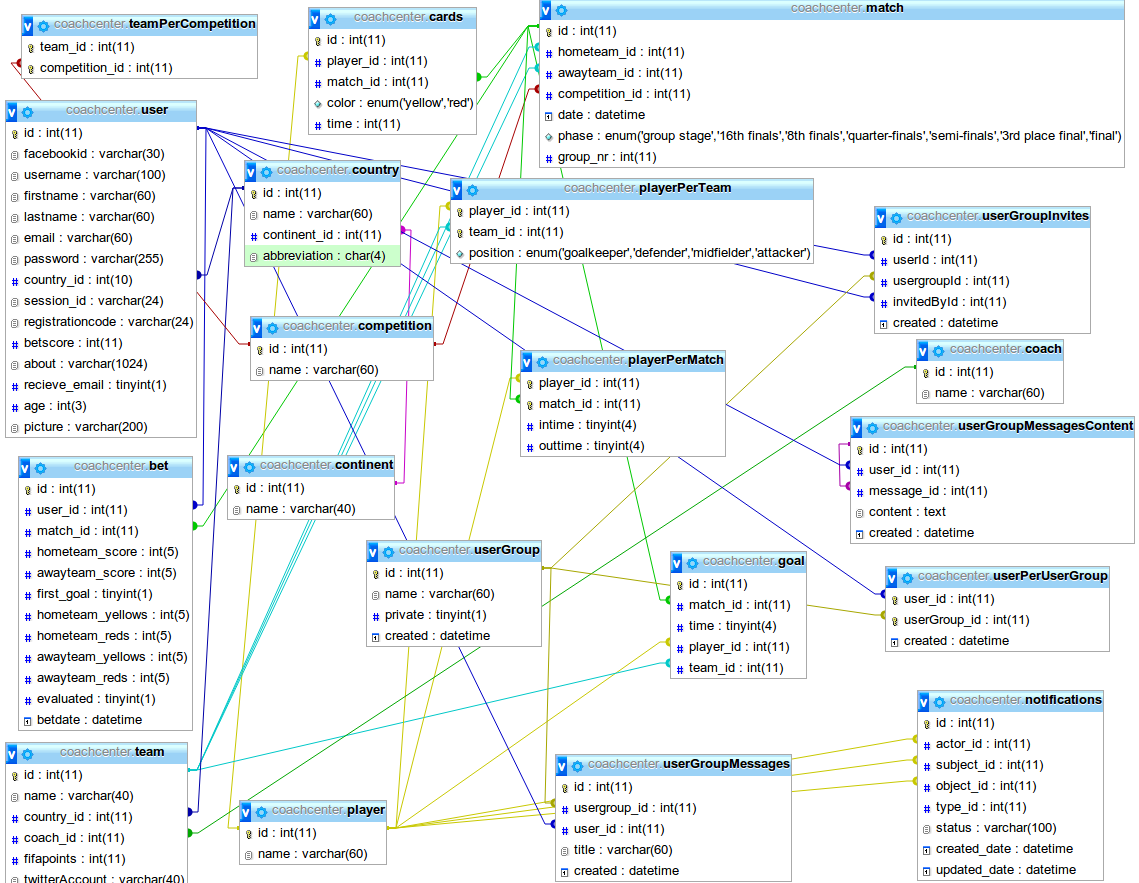
\includegraphics[width=90mm]{ER.png}
%\caption{Onze database in ER-model}
%\label{overflow}
%\end{figure}

\end{document}
